%
% This work is based on the samplepaper.tex template.
% Version 2.20 of 2017/10/04
%

\documentclass[runningheads]{llncs}
\renewcommand{\thesection}{\Roman{section}}

\usepackage[dvipsnames]{xcolor}
\usepackage{graphicx}
\usepackage{color}
\usepackage[colorinlistoftodos]{todonotes}
\usepackage[normalem]{ulem}
\usepackage[acronym]{glossaries}
\usepackage{xargs}
\usepackage[utf8]{inputenc}

\inputencoding{utf8}

% @Cristian You can you use this kind of stuff to define your own TODO colors,
% and then it's easy to call from text. Like this:
% \todoglg{<some text>}

\newcommandx{\todoglg}[2][1=]{\todo[
	linecolor=ForestGreen,
	backgroundcolor=ForestGreen!25,
	bordercolor=ForestGreen,
	#1]{#2}}
\newcommandx{\todoam}[1]{\todo[
	linecolor=red,
	backgroundcolor=red!25,
	bordercolor=red]{#1}}

% If you use the hyperref package, please uncomment the following line
% to display URLs in blue roman font according to Springer's eBook style:
% \renewcommand\UrlFont{\color{blue}\rmfamily}

\begin{document}

\title{Wireless Network for In-Car Communication}
%
%\titlerunning{Abbreviated paper title}
% If the paper title is too long for the running head, you can set
% an abbreviated paper title here
%

\author{Cristian Alderete \and
Guillaume Le Gall \and
Alexandre Marquet \and \\
Georgios Z. Papadopoulos \and
Nicolas Montavont
}
%
\authorrunning{C. Alderete et al.}
% First names are abbreviated in the running head.
% If there are more than two authors, 'et al.' is used.
%
\institute{IMT Atlantique, IRISA, UBL, France \\
%2, rue de la Châtaigneraie, \\
%35576 Cesson S\'evign\'e, France \\
\email{firstname.lastname@imt-atlantique.fr}}
%
\maketitle              % typeset the header of the contribution
%

% List of acronyms.
\newacronym{osv}{OSV}{Open-Source Vehicle}
\newacronym{iot}{IoT}{Internet of Thing}
\newacronym{can}{CAN}{Controller Area Network}
\newacronym{bms}{BMS}{Battery Management System}
\newacronym{ec}{EC}{Engine Controller}
\newacronym{soc}{SOC}{State of Charge}
\newacronym{wsn}{WSN}{Wireless Sensor Network}
\newacronym{coap}{CoAP}{Constrained Application Protocol}
\newacronym{rest}{REST}{Representational State Transfer}
\newacronym{uart}{UART}{Universal Asynchronous Receiver-Transmitter}
\newacronym{lln}{LLN}{Low-Power Lossy-Network}
\newacronym{rpl}{RPL}{Routing Protocol for Low-Power and Lossy Networks}
\newacronym{pwm}{PWM}{Pulse-Width Modulation}
\newacronym{api}{API}{Application Programming Interface}
\newacronym{i2c}{I2C}{Inter-Integrated Circuit}
\newacronym{mac}{MAC}{Medium Access Control}

\begin{abstract}

%\todoglg{We are missing the idea that wireless links are already used in cars for tire pressure monitoring.}

In this demo, we present a framework to retrieve data from an electric vehicle platform and publish it through an embedded wireless network. 
We developed driver programs to read the car's data (such as speed, battery level, etc.), and
we built a IEEE802.15.4-TSCH network with a \gls{coap} server to make it available to other devices.
We also developed a dashboard, including a \gls{coap} client, and multiple displays, to show the relevant information in real time to the driver.

\keywords{Electric vehicle \and IoT \and In-car Networking \and 802.15.4 \and 6TiSCH \and CoAP}

\end{abstract}
%

\section{Introduction}
\label{sec:intro}

About two decades from now, automotive manufacturers have moved away from point to point links for in-car communications.
They switched to using embedded buses such as \gls{can} to provide the on-board devices with a communication network.
This was a first step towards cost, weight and complexity reduction in communication systems.
With the emergence of \gls{wsn} technologies, research effort is being made to introduce them for in-car communications \cite{Bi2015},~\cite{Huang2018}.


With this in mind, we developed a proof-of-concept of a car network backbone, based on the \gls{osv} electric car platform \cite{open-motors-tabby}.
Our goal is to retrieve the relevant data from the main devices of the vehicle and make it available to a low power and highly reliable wireless network.
To this extent, we use state of the art \gls{iot} protocols.
Finally, we display this data to the driver via a dashboard.


As we believe layer 2 \gls{mac} scheduling will be one of the keys to a reliable wireless network, our effort will be centered around using and improving the IEEE 802.15.4-TSCH MAC layer for our communicating devices.

\section{Architecture and Protocols}

\subsection{The Open-Source Vehicle electric car}
\label{subsec:osv}

\subsubsection{Platform}

%Introduction to OSV (the one we use, in particular).
This demonstration is based on the Tabby Evo \gls{osv}, from Open Motors.
%\footnote{\url{https://www.openmotors.co/osv-platform/}, \url{https://elinux.org/OSVehicle}}.
%,~\cite{elinux-osvehicle}.
We chose this platform due to its simplicity and because it offers a ground for add-ons, enhancements and concept demonstrations.
As a vehicle platform, it only captures the essence of an actual car: it has
no car body, nor any indicator and, in particular, no dashboard.

Our work is mainly focused on the \gls{osv} powertrain.
This comprises every system involved in generating power and transforming it
into mechanical forces, such as: the Lithium-Ion battery, the \gls{bms}, the
\gls{ec} -- or inverter -- and the electric 3-phase AC engine.
The \gls{ec} and the \gls{bms} are the main devices that guarantee the safe and reliable operation of the powertrain.

The \gls{bms} handles the measurement of battery parameters, such as cells voltages, current, temperature, and calculates the \gls{soc}. 
Then, from all this information, it enables or disables the on-board charger and
\gls{ec}.
This way, it ensures that the battery cells remain in their safety window (\textit{i.e.}, their allowed voltage and temperature range).


The \gls{ec}'s purpose is to generate the 3-phase AC current to run the engine and control its magnitude and frequency through a feedback loop.

These two core components hold important data about the vehicle, and are capable of exposing them to other devices, as depicted in Figure~\ref{platform}.

\begin{figure}[!h]
	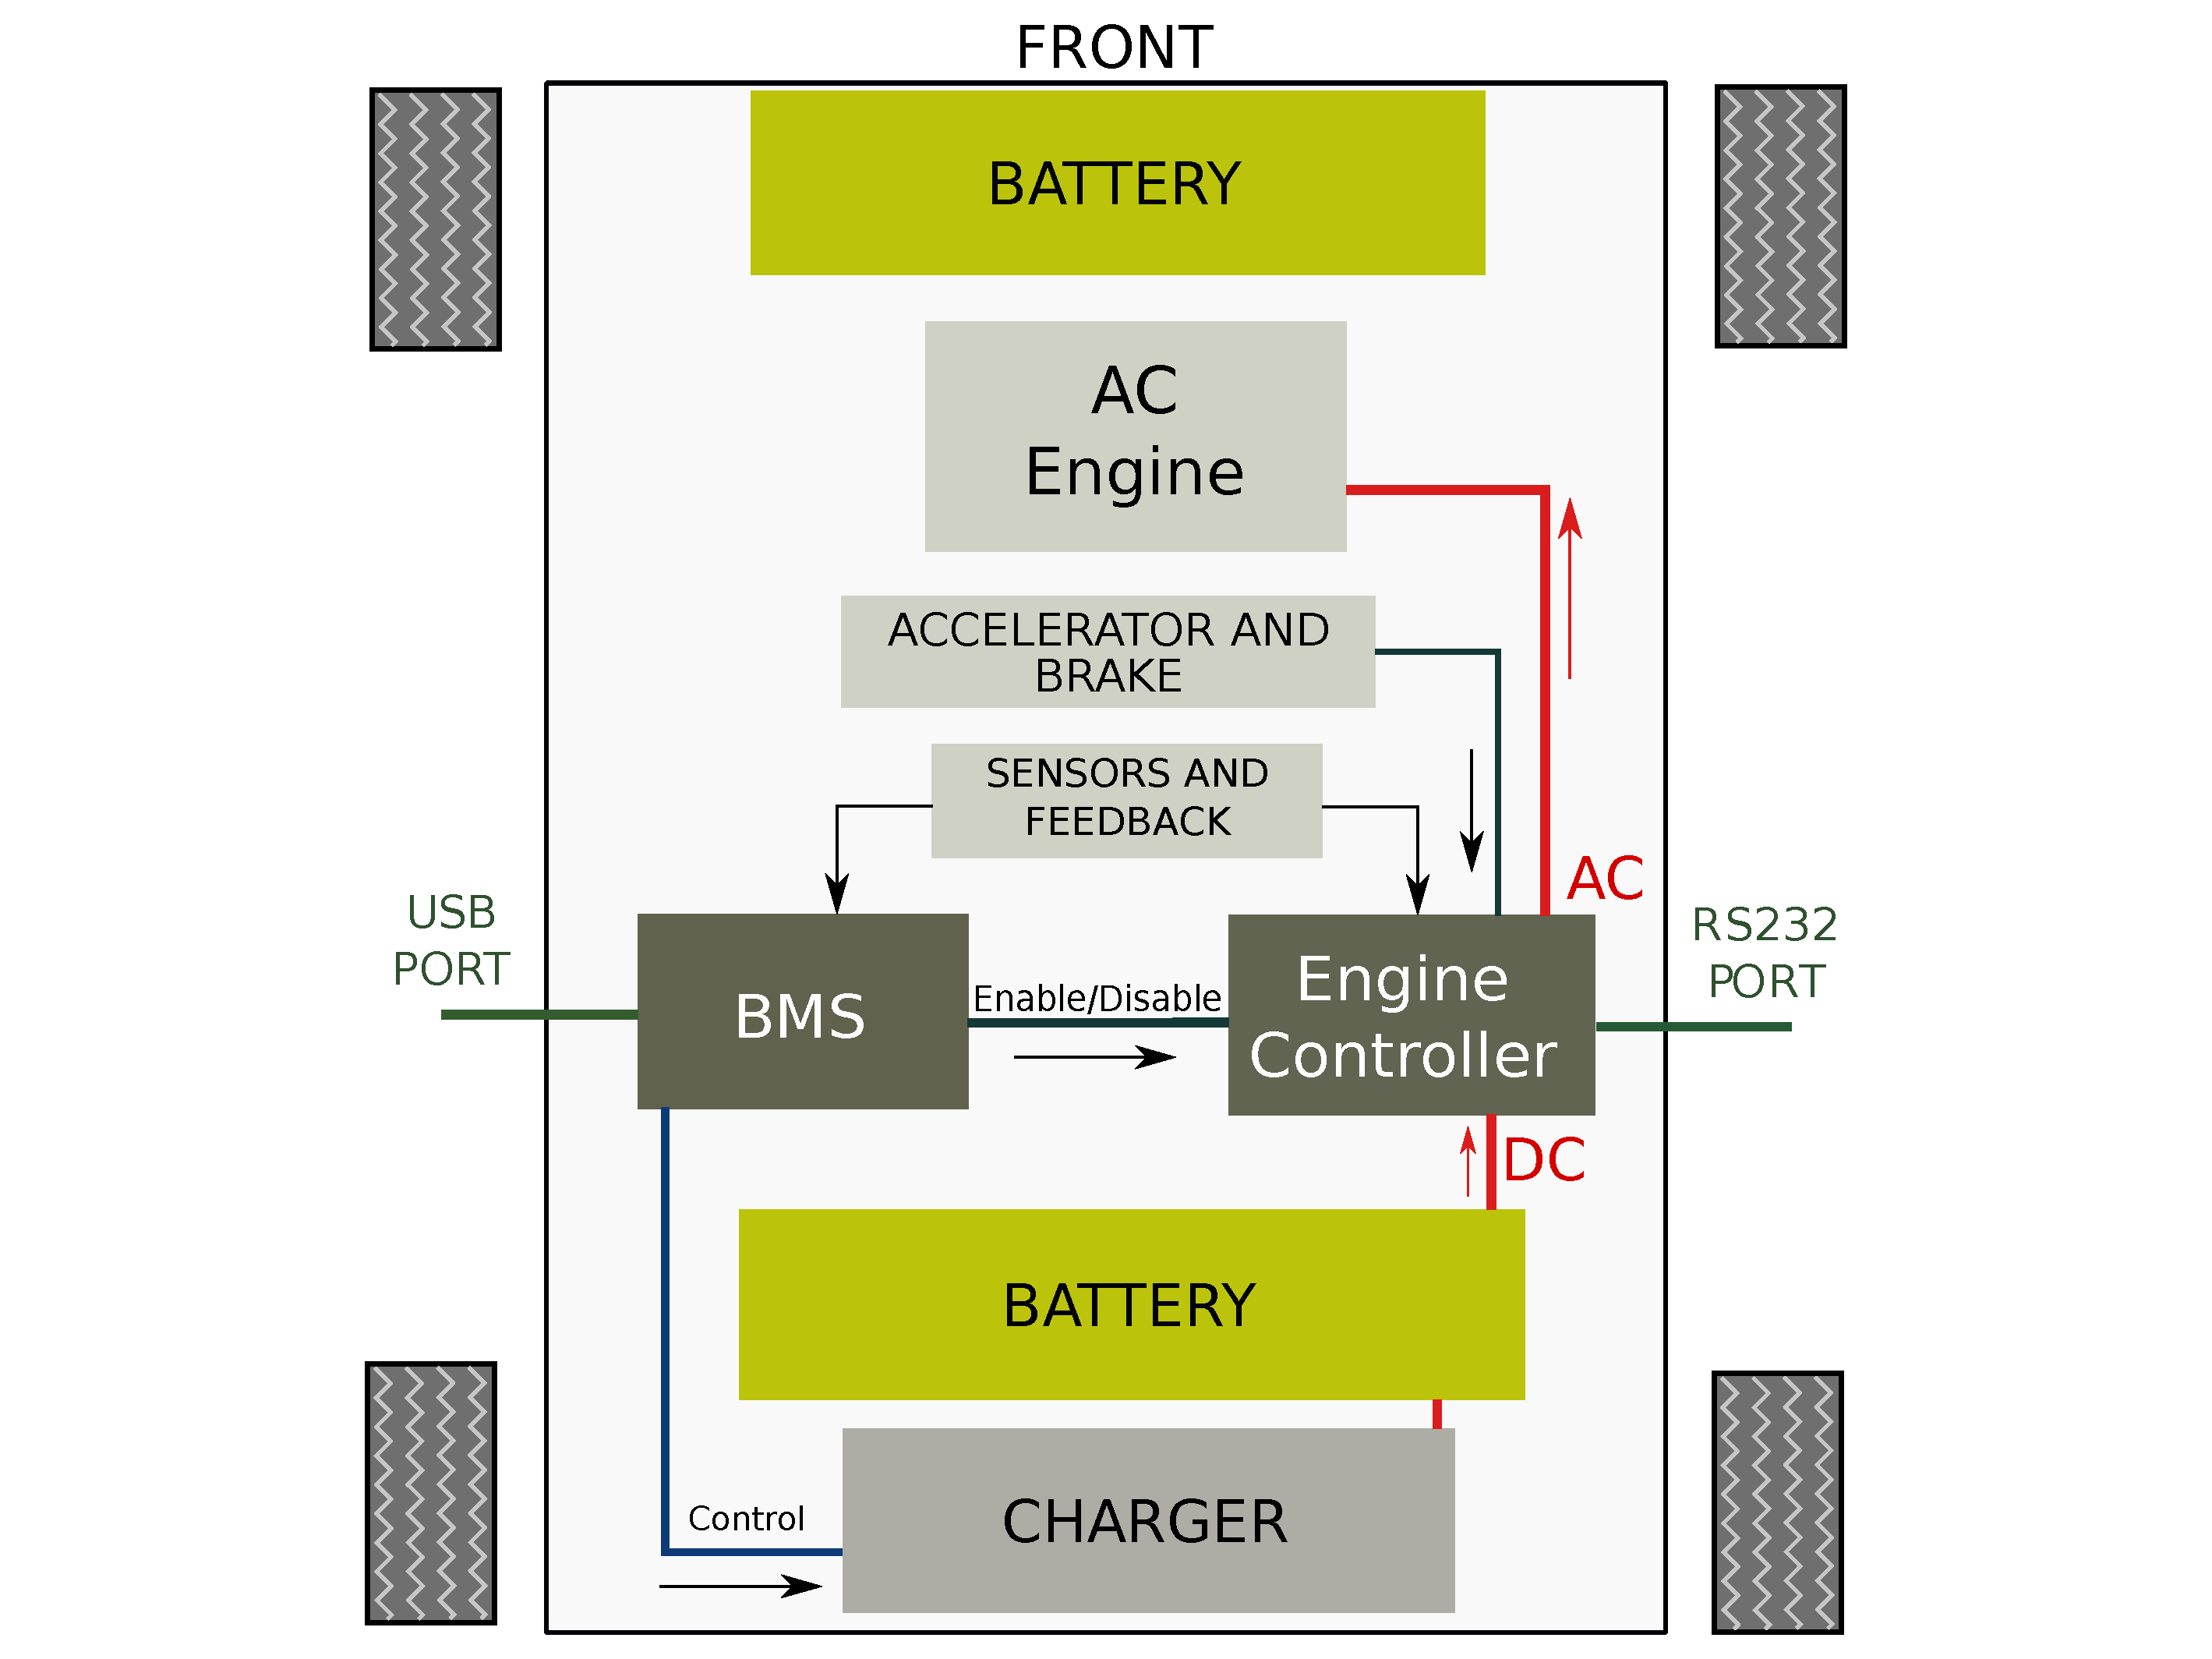
\includegraphics[width=\textwidth]{OSV.pdf}
	\caption{\gls{osv} powertrain functional overview.}
	\label{platform}
\end{figure}


\subsubsection{Available Data}

On the \gls{osv} platform, most of the relevant data can be retrieved from the \gls{bms} and \gls{ec}.
Some of it should be exposed to the
driver in real time (like the speed of the car, or the battery \gls{soc}), while the rest of it can be displayed on-demand (e.g., for maintenance).
Table \ref{tab:data} shows the selected data for this demonstration.
Even though this information is generated within the \gls{osv}, 
the original platform lacks displays to show it.

Both the \gls{bms} and \gls{ec} expose their available data through a custom
ad-hoc protocol built on top of a \gls{uart} connection.
Each component implements its own protocol and data format.
The \gls{bms} protocol is a simple enable/disable data flow model: data stream
starts when the reader device sends an ``enable'' command, and stops when a
``disable'' command is sent.
This has the disadvantage of being forced to request the entire set of variables when just a few are needed.
On the other hand, the \gls{ec} implements a request/response communication
protocol, meaning that each variable is requested separately with a specific
command.

The stock system requires point to point connections to the \gls{bms} and \gls{ec} which prevents easy spreading of information within the vehicle.
This is why we build an in-vehicle wireless network: to make the powertrain's data available to the rest of the vehicle.



\subsection{Wireless Network Protocol Stack}
\label{subsec:protocol-stack}

One of the motivations of this work is to break the link between data generation and data consumption with an embedded wireless network.
Exposing the data through a \gls{rest} \gls{api} allows for enhanced usage.


In this context, and within a \gls{wsn}, \gls{coap} is the preferred application-layer protocol \cite{RFC7252}.
It provides a request/response model between two endpoints, using a subset of HTTP request methods such as GET, PUT, POST and DELETE \cite{RFC7231}.
Furthermore, \gls{coap} offers extensions such as OBSERVE which allows the
client to subscribe to resources on a server and get notified upon changes.


The CoAP standard runs over UDP as the transport layer.
At the network layer, we deploy a 6LoWPAN IPv6 network \cite{RFC4944}.
With an eye towards optimizing the constrained network, the 6TiSCH mode of
the link-layer and physical layer protocol IEEE 802.15.4e is used \cite{RFC8180},~\cite{802-15-4}.
Along the same line, the \gls{rpl} handles IP routing \cite{RFC6550}.


\subsection{Proposed Architecture}
<<<<<<< HEAD
% HOW DO I MAKE IT AVAILABLE!??  (NOT TALK ABOUT OPENMOTE or HARDWARE.. contiki
% either )
 
Figure \ref{car_network} illustrates the functional diagram of the proposed
=======

Figure~\ref{car_network} illustrates the functional diagram of the proposed
>>>>>>> aa8560b95678d29daef37270ba837199baca2dc8
architecture.
In this scenario, we distinguish two main blocks that communicate through a wireless network: the transmitter and the receiver.
On the transmitter side, the information from the powertrain is retrieved,
processed and then stored in the \gls{coap} server.
On the receiver side, the client requests information using GET or OBSERVE \gls{coap} methods, and forwards it to the display handler.

\begin{figure}[!h]
	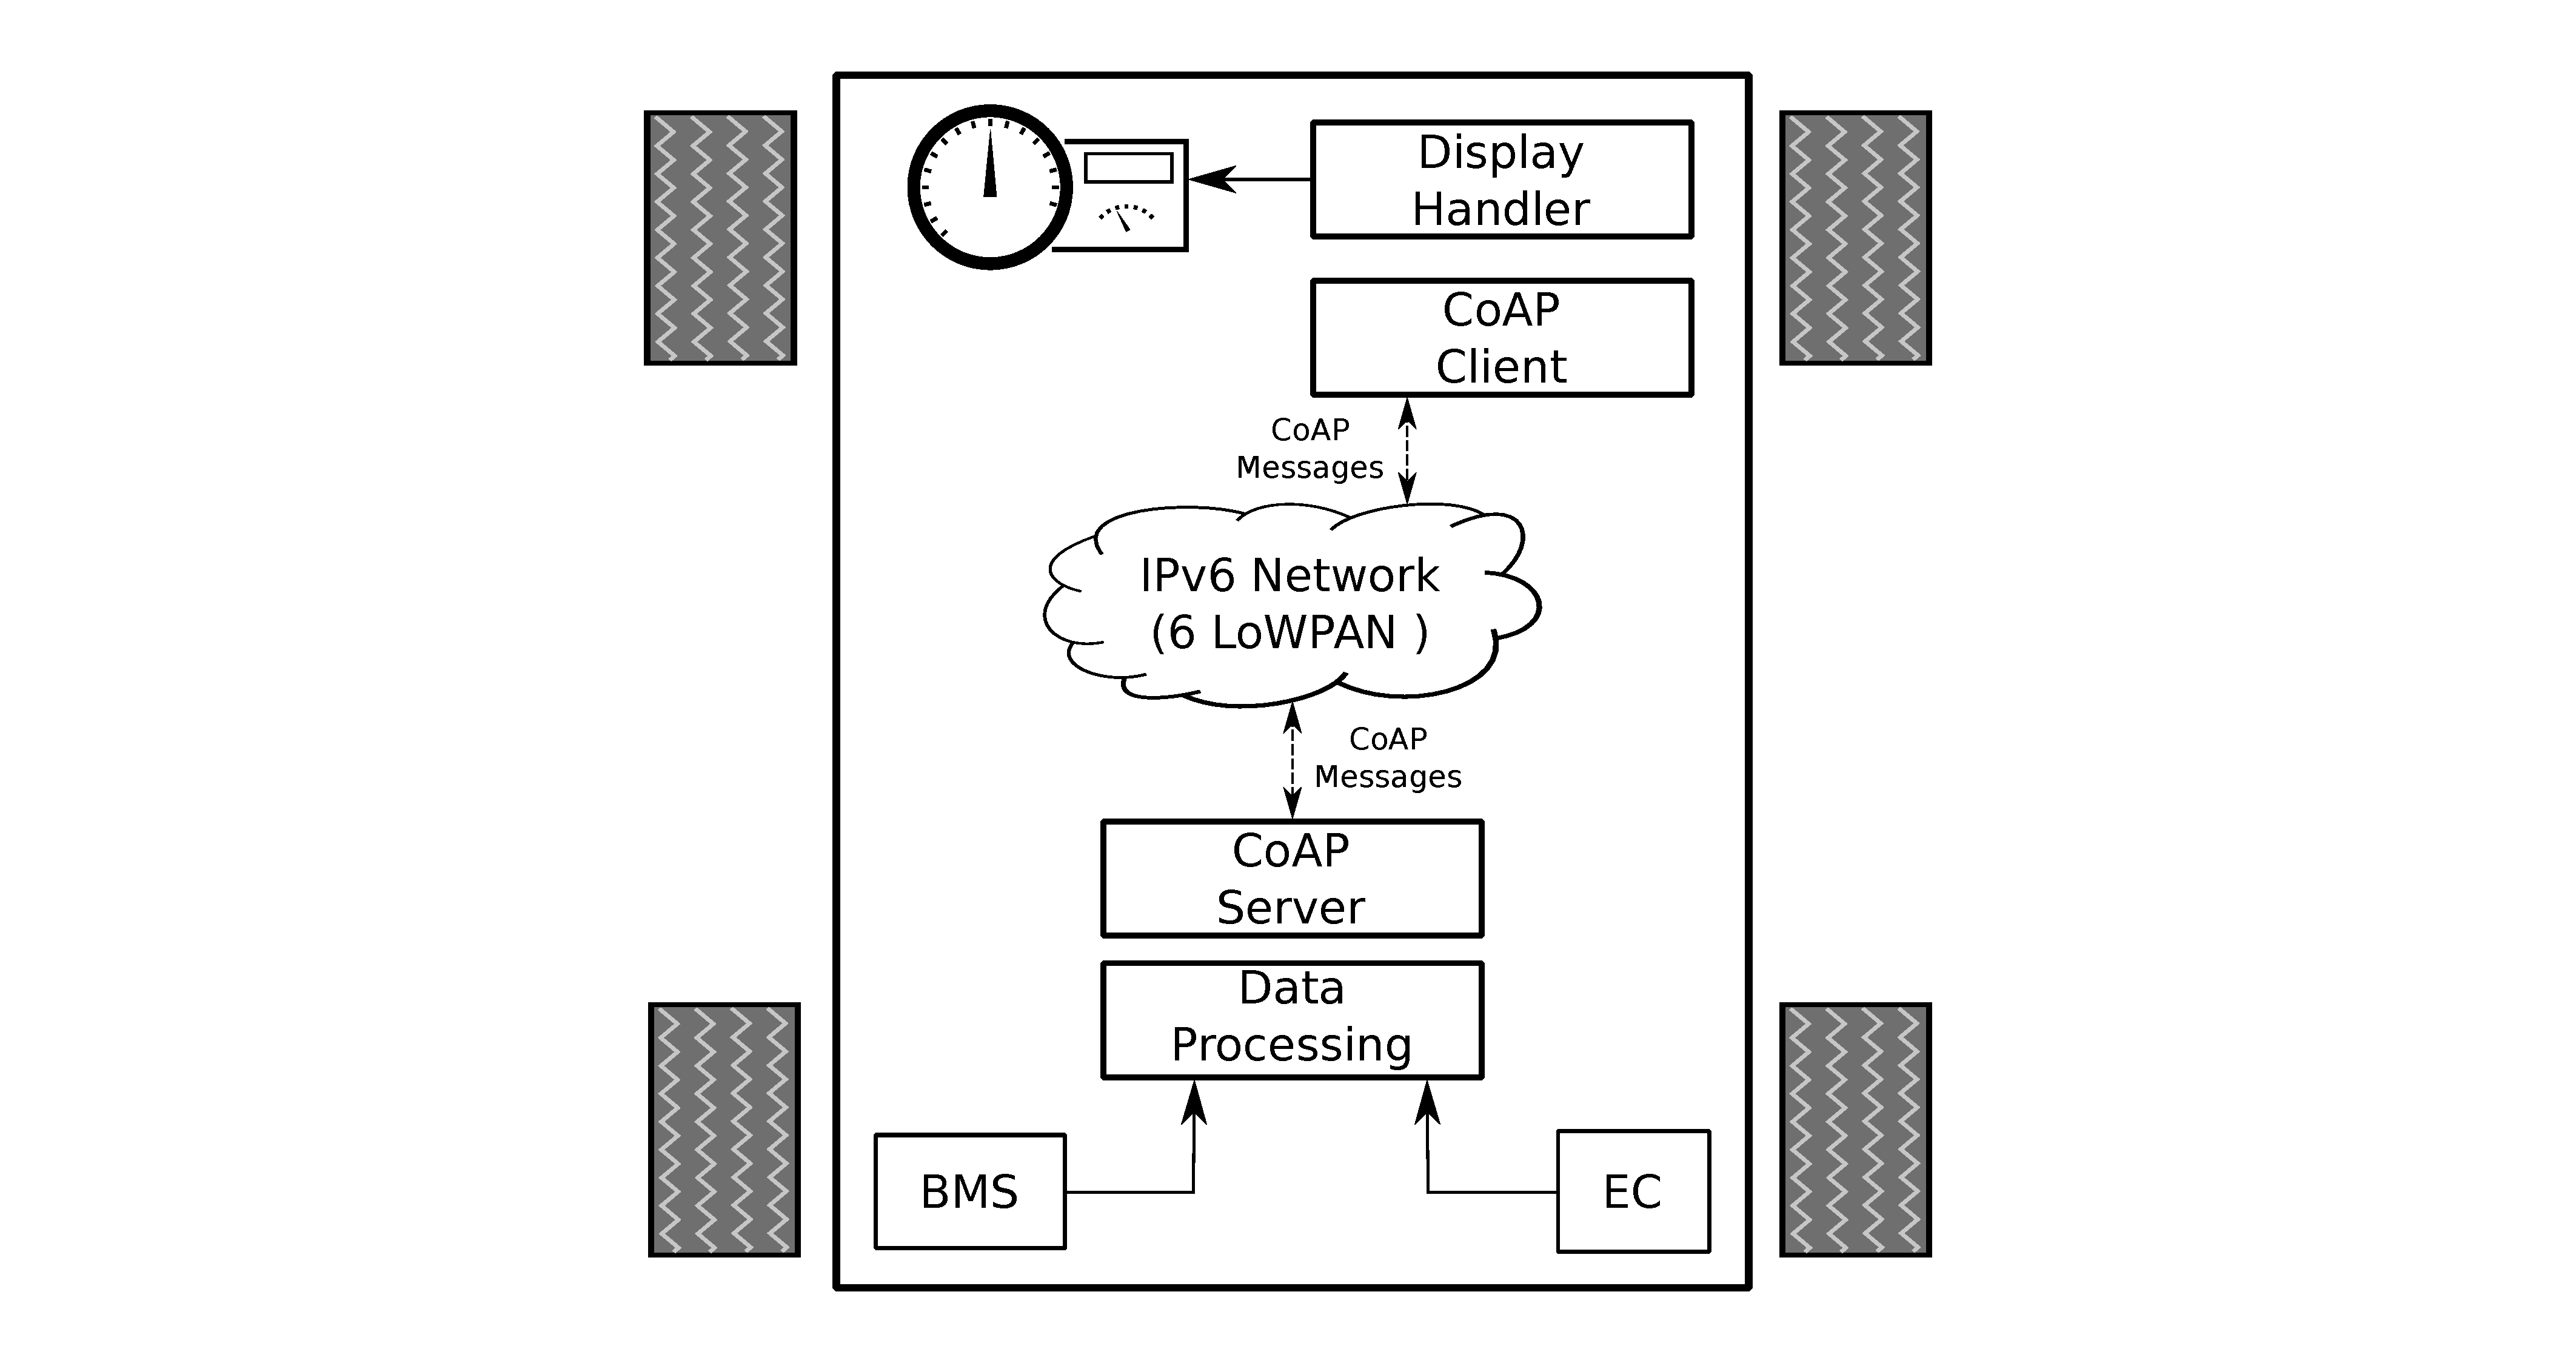
\includegraphics[width=\textwidth] {Car_Network.pdf}
	\caption{Data flow from \gls{bms} and \gls{ec} to the dashboard.}
	\label{car_network}
\end{figure}


\section{Demonstration}
\label{sec:demo}

\subsection{Hardware}
\label{subsec:hardware}

As an implementation of the ideas presented so far, we develop the
full architecture shown in Figure~\ref{full_architecture}, which shows the
hardware as well as the involved protocols.
As a display handler, we use an Arduino UNO board, since it can natively handle \gls{uart} and \gls{i2c} protocols, as well as \gls{pwm} signals, which are needed by the different displays we use.
For data collection and processing, we use an Arduino DUE because it has a 
more powerful micro-controller that supports USB hosting to communicate with the
\gls{bms}.
For the wireless communication, we use two OpenMotes CC2538 transceivers.
These low power modules, running the Contiki Operating System, use IEEE
802.15.4 and support the protocol stack proposed in section
\ref{subsec:protocol-stack}.
Additionally, they provide serial ports that are used to communicate with the Arduino boards.
Finally, note that voltage shifters are needed to avoid voltage level mismatches when interconnecting the chosen hardware.
More details on hardware role and connections can be found in Table
\ref{hardware}. 


\begin{figure}[!t]
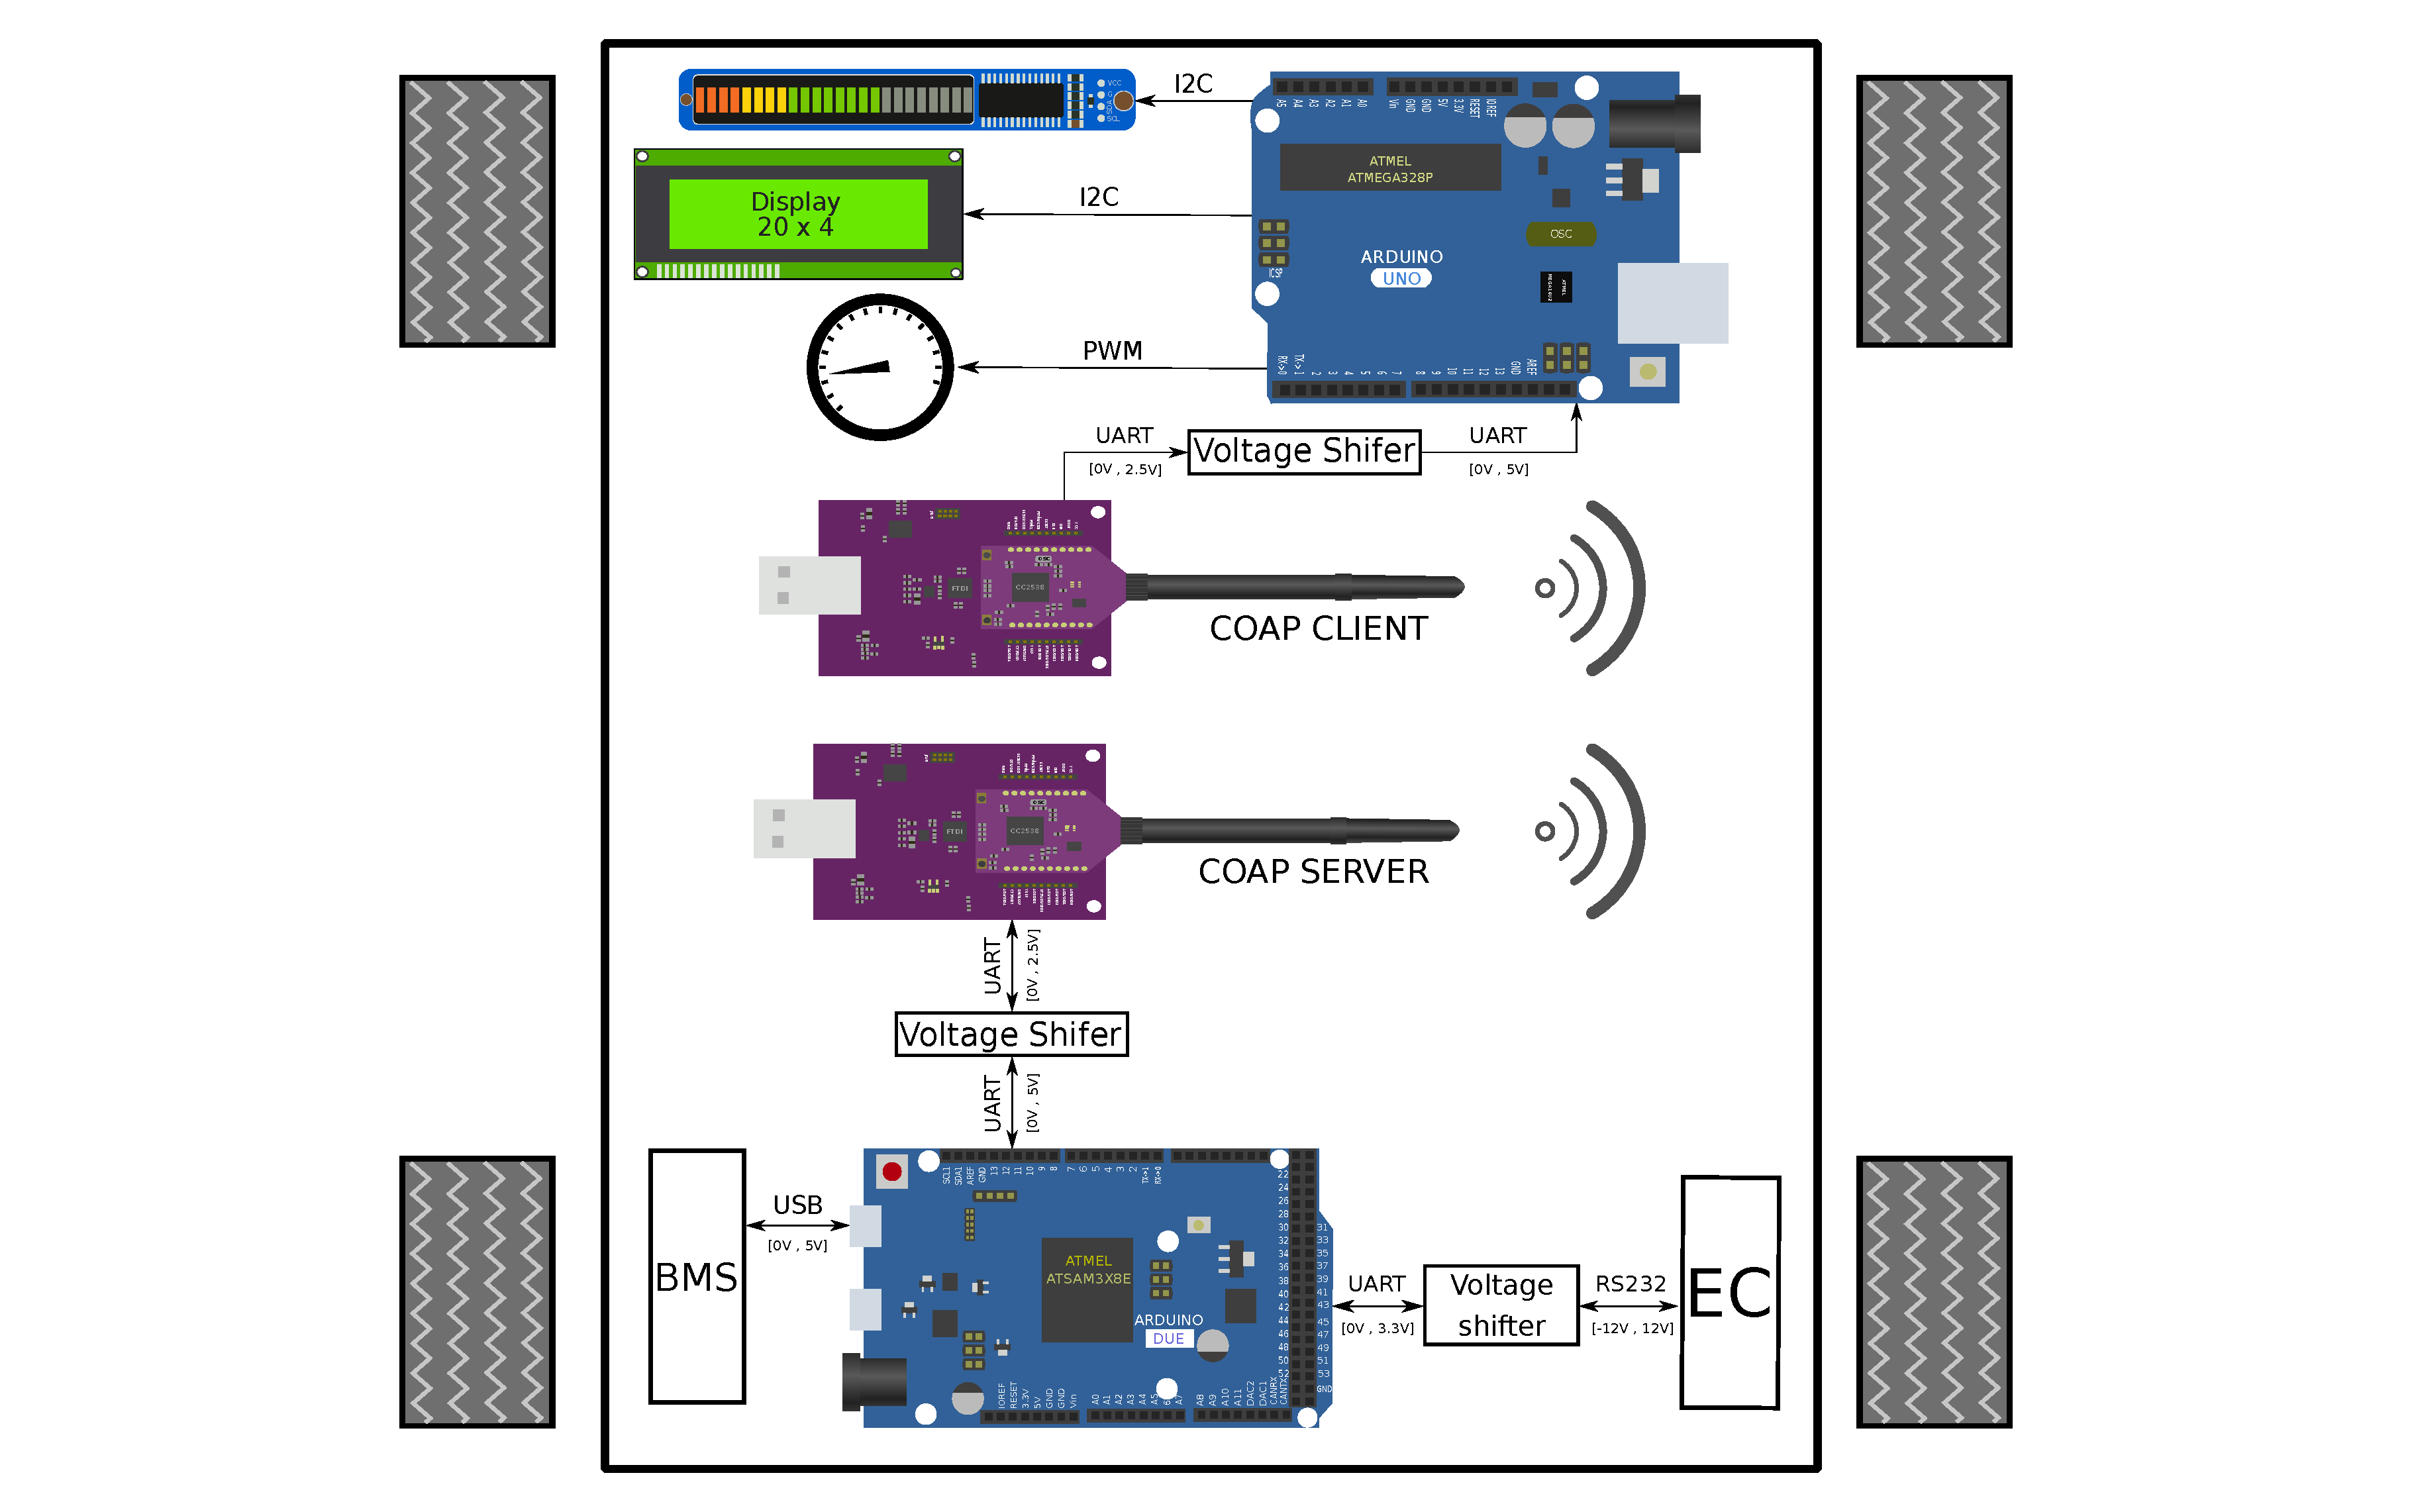
\includegraphics[width=\textwidth] {proposed_architecture.pdf}

\caption{Proposed architecture for this demonstration.} \label{full_architecture}
\end{figure}

\begin{table}[!t]
	\centering
	\caption{Hardware used in the demonstration.}\label{hardware}
	\begin{tabular}{|l|l|l|}
		\hline
		Device & Ports used  &  { Main Task } \\
		\hline
		
		Arduino DUE  &  { UART1/I2C/USB-host }  &  { Interface }  \\
		Arduino UNO &  { UART1/UART2/PWM/I2C } &  { Display Handler }\\
		Openmote CC2538 REV-A1 & { I2C } &  { Transmitter }\\
		Openmote CC2538 REV-A1 & { UART } &  { Receiver } \\
		LCD Display & { I2C } &  { Display Km,$^{\circ}C$, V}\\
		Servo-motor & { PWM }  &  { Display Km/h }\\
		Bar Led Display & { UART } &  { Display SoC}  \\
		\hline
		
	\end{tabular}
\end{table}

\begin{table}[!t]
	\centering
	\caption{Resources Management.}\label{resources}\label{tab:data}
	\begin{tabular}{|l|l|l|l|}
		\hline
		Resource & Origin  & Request type & Server Update Strategy\\
		\hline
		
		Speed &  \gls{ec} & OBSERVE & Conditioned by Charging \\
		SoC  & \gls{bms} & OBSERVE& Conditioned by Speed and Charging\\
		Distance & \gls{ec} & OBSERVE & Conditioned by Speed\\
		Charging & \gls{bms}  & OBSERVE & Conditioned by Speed\\
		Temperature & \gls{bms}  & OBSERVE & Periodically \\
		Cells Voltages & \gls{bms}  & GET & Periodically \\
		\hline
	\end{tabular}
\end{table}


\subsection{Resource Management}
\label{subsec:ressource-mgmt}


In order to address the trade-off between data freshness and network usage, 
we take advantage of the OBSERVE \gls{coap} feature.
This allows the server to immediately notify the client when resources are
updated instead of having periodic requests, thus reducing the network stress.
Also, using this feature we can focus on optimizing when and how to update the
server, knowing that the observing client will be automatically notified.


For this purpose, we implement an updating policy in the server, based on key relationships between the resources.
For example, the \gls{coap} server waits for the car to move to update
the traveled distance, or similarly it does not update
the speed if the vehicle is charging.
Furthermore, we establish minimum thresholds to guarantee that the updated value
has a relevant difference with the previous one before notifying clients.
For demonstration purposes, we also implement the GET method to request the cells voltages. Table \ref{resources} sums up the monitored resources.





\section{Conclusion}

In this demo, we presented what is the starting point of a car network backbone using state of the art \gls{wsn} technologies, on top of a simple electric car platform.
We retrieved some data from the core devices of the powertrain, and exposed them with a standard \gls{api}.
We also made a dashboard, which consumes this data.

We believe that the concepts brought by the \gls{rpl} and \gls{coap} protocols can lead to more flexible design for in-car communications.
Wireless links also provide the benefits of cost and weight reduction.
In the future, even though \gls{wsn} will probably not become the default technology used for cars network backbone, they could be complementary to a wired solution, mainly for monitoring or non-critical applications.

Furthermore, our set-up is a starting point to evaluate the performances of in-car wireless networks and how the 802.15.4-TSCH scheduler and \gls{rpl} can be optimized for such networks.


\bibliographystyle{splncs04}
\bibliography{references}

\end{document}

